\section{vServer}\label{subsec:vserver}

In diesem Kapitel wird auf den Betrieb eines vServers eingegangen, auf dem die Docker-Umgebung anschließend öffentlich zugänglich gemacht werden soll.
Neben der Bereitstellung des vServers wird auch auf die Automatisierung von Updates und die Verwendung eines Reverse Proxys eingegangen.

\subsection{Hosting}\label{subsubsec:hosting}

Im Laufe des Projektes wurde die Idee geboren, einen vServer zu mieten, um die Docker-Container öffentlich zugänglich zu machen und damit von überall aus auf Collectiqo zugreifen zu können.
Hierzu wurde ein vServer bei dem Hostinganbieter netcup GmbH gemietet, der im Rechenzentrum-Standort Nürnberg betrieben wird.
Konkret handelt es sich um das Produkt \textit{VPS 1000 ARM G11}, einen vServer auf ARM-Basis mit 6 vCores, 8 GB RAM, 256 GB NVMe Speicher und einer 2500 Mbit/s Anbindung.
Hierfür ist eine IPv4-Adresse und ein /64-Netz für IPv6-Adressen inkludiert.

Zwecks einfachem Zugriff Richtung Server wurden ebenfalls zwei Domains bei der netcup GmbH registriert.
Hierbei handelt es sich um die Domains \textit{collectiqo.de} und \textit{collectiqo.com}, die mittels DNS-A-Record auf die IPv4-Adresse 89.58.44.11 des vServers zeigen.

Als Betriebssystem wurde \textit{Ubuntu Server 24.04 LTS minimal with ssh} als Installation gewählt.
Alle notwendigen Dienste und Softwarepakete werden somit nachträglich installiert.
Der Zugriff auf den Server erfolgt mittels SSH und einem privaten Schlüssel, der auf dem lokalen Rechner hinterlegt ist.

\subsection{Automatisierung Updates}\label{subsubsec:automatisierung-updates}

Um den Server zu härten und eine fortlaufende Sicherheit zu gewährleisten, werden Updates automatisiert durchgeführt.
Hierzu wurde das Paket \textit{unattended-upgrades} konfiguriert, welches in Debian-basierten Distributionen, wie u.\,a.\ Ubuntu, enthalten ist.
Durch die Konfiguration des Paketes \textit{(/etc/apt/apt.conf.d/50unattended-upgrades)} wird sichergestellt, dass der Server täglich nach Updates sucht und diese installiert.
Dies betrifft sowohl Sicherheitsupdates als auch Updates für installierte Softwarepakete.
Sollte ein Neustart des Servers notwendig sein, wird dieser ebenfalls automatisiert durchgeführt.
Der Zeitpunkt der Einspielung der Updates beziehungsweise des Neustarts wurde auf 6 Uhr morgens festgelegt.
Somit ist gewährleistet, dass der Server stets ohne händische Eingriffe auf dem neuesten Stand ist.

Um über den Status der Updates informiert zu sein, wurde eine E-Mail-Benachrichtigung eingerichtet.
Hierzu wurden die Pakete \textit{apt-listchanges} sowie \textit{mailutils} installiert und \textit{Postfix}, ein Mail-Transfer-Agent für Unix-Derivate, konfiguriert.
In der Configuration-File \textit{(/etc/postfix/main.cf)} wurde die Domain \textit{collectiqo.de} gewählt.
Ebenso wurde mit dem Eintrag \textit{inet\_interfaces = loopback-only} die Konfiguration so angepasst, dass nur lokale Mails versendet werden können.
Der Empfang von Mails ist somit nicht möglich, es handelt sich damit um einen sogenannten send-only SMTP-Server.

\begin{figure}[h]
    \centering
    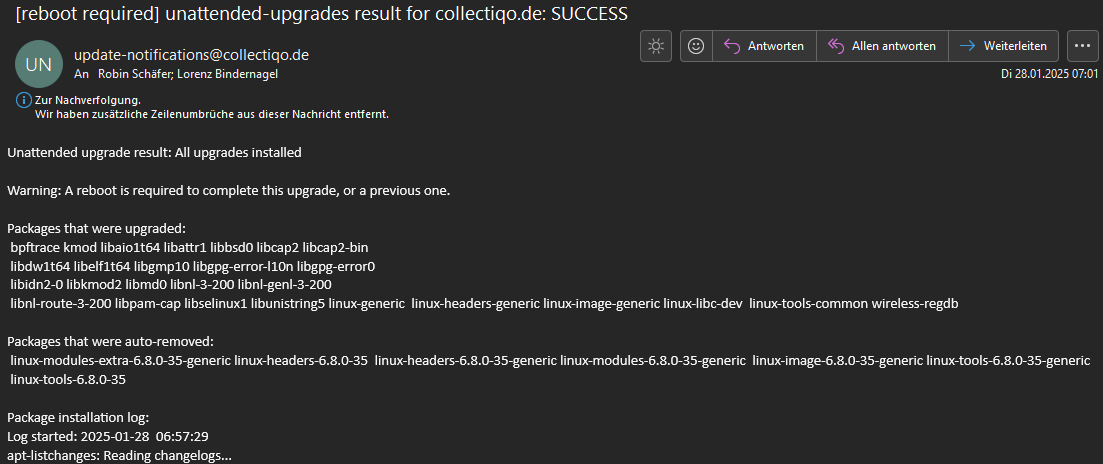
\includegraphics[width=0.9\textwidth]{update_notification}
    \caption{E-Mail Benachrichtigung bei Updates}
    \label{fig:update_notification}
\end{figure}

\begin{figure}[h]
    \centering
    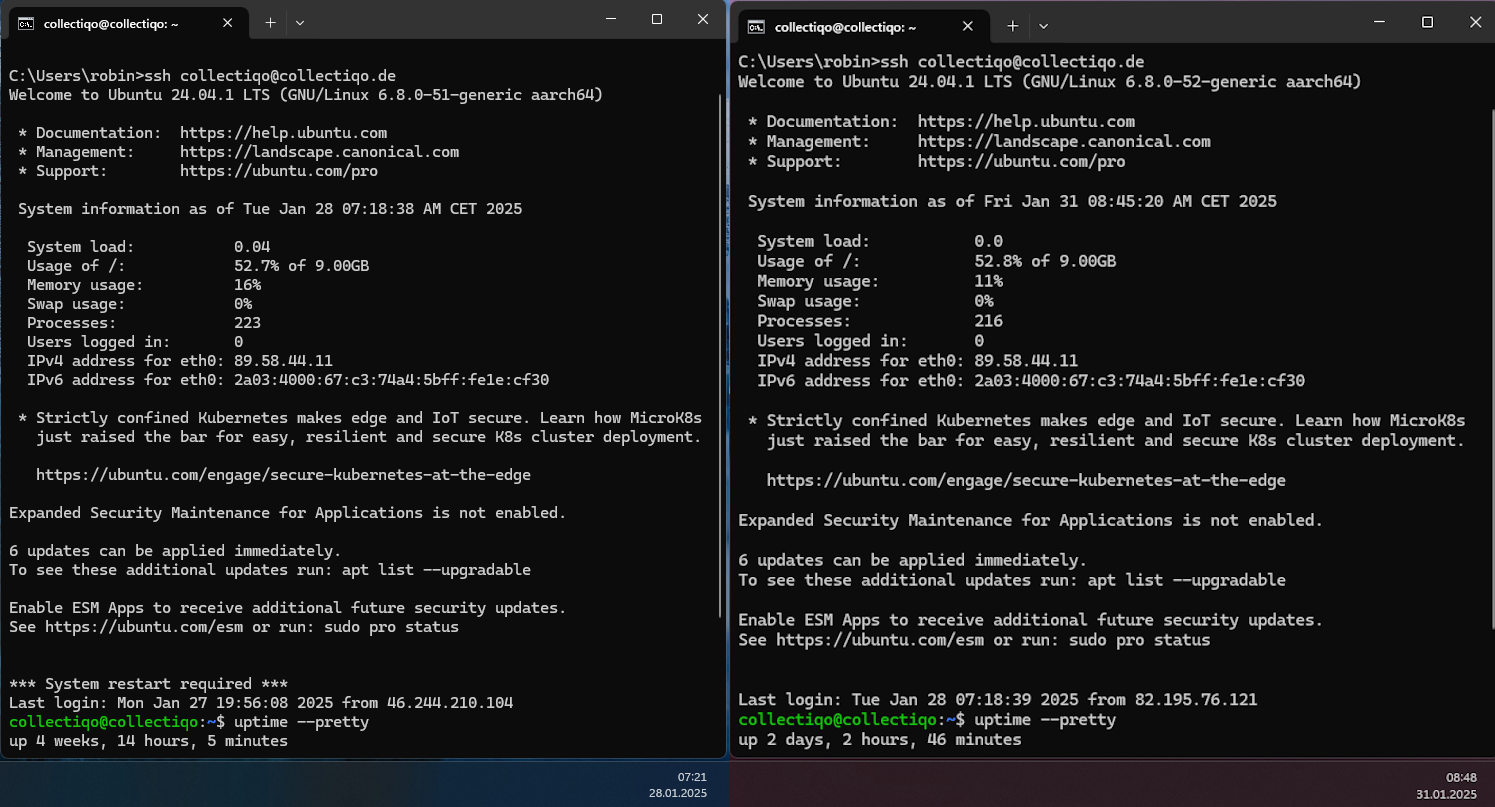
\includegraphics[width=0.9\textwidth]{update_autoreboot}
    \caption{Automatischer Neustart am daraufolgenden Morgen}
    \label{fig:update_autoreboot}
\end{figure}

\subsection{Reverse Proxy}\label{subsubsec:reverse-proxy}

Bei der Recherche, wie der integrierte Webserver innerhalb des node.js-Containers auf dem vServer mit einer verschlüsselten Verbindung über HTTPS öffentlich erreichbar gemacht werden kann, fiel schnell auf, dass dies ohne weitere Anpassungen nicht möglich ist.
Selbst signierte SSL-Zertifikate sind nicht ausreichend und vertrauenswürdig genug, um von den gängigen Webbrowsern akzeptiert zu werden.
Zudem ist eine automatisierte Ausstellung von Zertifikaten für den node.js-Container ohne weiteres ebenso nicht möglich.

Die Lösung hierfür ist die Verwendung eines Reverse Proxys, der als Zwischenstation zwischen dem node.js-Webserver und dem Client agiert.
Der Reverse Proxy ist für die Entgegennahme von Anfragen über das Internet zuständig und leitet diese an den node.js-Webserver weiter.
Er ist in der Lage, verschlüsselte Anfragen entgegenzunehmen, bevor diese ggf. unverschlüsselt intern an einen weiteren Webserver weitergeleitet werden.
Da bereits im Abschnitt \ref{subsec:implementierung-von-https} die Implementierung von HTTPS mittels eines selbst signierten Zertifikats für den Zugriff auf den node.js-Webserver beschrieben wurde, wird die Verbindung zwischen dem Reverse Proxy und node.js verschlüsselt weitergereicht.

Als Reverse Proxy wurde \textit{Nginx} gewählt, da dieser weit verbreitet ist und eine Vielzahl an Konfigurationsmöglichkeiten bietet.
Nginx wurde als weiterer Docker-Container erstellt und so konfiguriert, dass Anfragen über Port 80 und 443 der Domains \textit{collectiqo.de} und \textit{collectiqo.com} entgegengenommen werden.
Anfragen über Port 80 werden automatisch auf Port 443 weitergeleitet, um eine verschlüsselte Verbindung zu gewährleisten.
Es findet zudem jederzeit eine Umleitung auf die Domain \textit{collectiqo.com} statt, um mit einer einheitlichen Domain nach außen aufzutreten.
Der Webauftritt soll sich auf \textit{collectiqo.com} konzentrieren, während \textit{collectiqo.de} mehr der Administration dient.

Die Zertifikate für die Domains wurden über die Zertifikatsstelle \textit{Let's Encrypt} ausgestellt und in den Nginx-Container eingebunden.
Hierfür wurde das Tool \textit{Certbot} innerhalb eines eigenen Containers verwendet, welches die Zertifikate automatisiert ausstellt und über einen Volume-Mount an den Nginx-Container weitergibt.
Die Zertifikate haben eine Gültigkeit von 90 Tagen, eine automatisierte Erneuerung wird zeitnah implementiert, Vorbereitungen hierfür wurden bereits getroffen.

Zu Testzwecken wurde ein dedizierter Webserver als Test-Webserver in einem separaten Container eingerichtet, um die Funktionalität des Reverse Proxys zu überprüfen, ehe dieser auf den node.js-Webserver umgeleitet wurde.
\textit{arm64v8/httpd} innerhalb Docker Hub basiert dabei auf \textit{apache}.
Eine einfache HTML-Datei wurde hierfür im Git-Repository abgelegt und als Volume-Mount an den Container übergeben.

Die Konfiguration des Nginx-Revers-Proxys erfolgte in der Datei \textit{nginx/nginx.conf} und sieht wie folgt aus:
\vspace{1em}
\begin{lstlisting}[label={lst:lst-nginx-config}]
events {
    worker_connections  1024;
}

http {
    server_tokens off;
    charset utf-8;
    server {
        listen 80 default_server;
        server_name collectiqo.de www.collectiqo.de collectiqo.com www.collectiqo.com;

        location ~ /.well-known/acme-challenge/ {
            root /var/www/certbot;
        }

        location / {
            return 301 https://collectiqo.com$request_uri;
        }
    }
    server {
        listen 443 ssl;
        server_name collectiqo.de www.collectiqo.de collectiqo.com www.collectiqo.com;

        ssl_certificate /etc/letsencrypt/live/collectiqo.com/fullchain.pem;
        ssl_certificate_key /etc/letsencrypt/live/collectiqo.com/privkey.pem;

        location ~ /.well-known/acme-challenge/ {
            root /var/www/certbot;
        }
        location / {
            #proxy_pass http://test-webserver;
            proxy_pass https://collectiqo-web-1:3000;
            proxy_http_version 1.1;
            proxy_set_header Host $host;
            proxy_set_header Upgrade $http_upgrade;
            proxy_set_header Connection 'upgrade';
            proxy_set_header X-Real-IP $remote_addr;
            proxy_set_header X-Forwarded-For $proxy_add_x_forwarded_for;
            proxy_set_header X-Forwarded-Proto $scheme;
            proxy_cache_bypass $http_upgrade;
        }
    }
}
\end{lstlisting}
\vspace{1em}
